\section{引导}

\begin{itemize}
\item bootloader是什么?
\item bootloader做了哪些事情?
\item xv6是如何被加载并启动的?
\item xv6如何实现内核态到用户态的转变的?
\item xv6启动用户态进程前需要完成哪些事情?
\end{itemize}

\subsection{开始}

当计算机加电后,一般不直接执行操作系统,而是执行引导加载程序。简单地说,引导加载程序就是在操作系统内核运行之前运行的一段小程序。通过这段小程序,我们可以初始化硬件设备、建立系统的内存空间映射图,从而将系统的软硬件环境带到一个合适的状态,以便为最终调用操作系统内核准备好正确的环境。最终引导加载程序把操作系统内核映像加载到RAM中,并将系统控制权传递给它。下面是一个通用操作系统的启动过程。

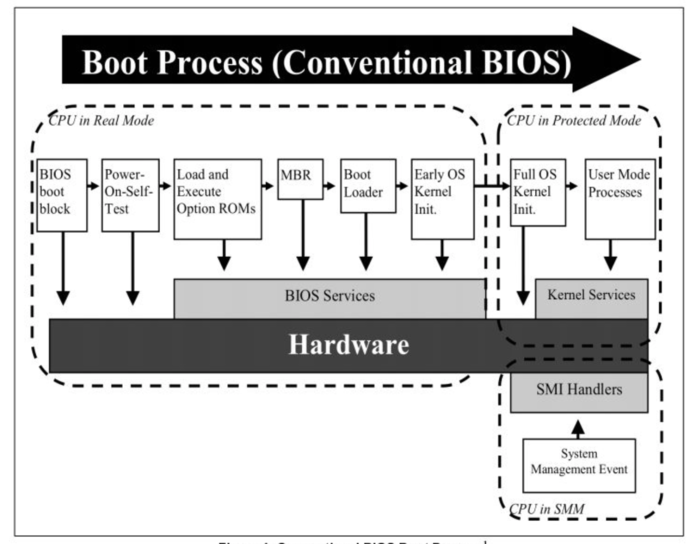
\includegraphics[width=6in]{figures/boot/fig1.png}


引导加载程序(bootloader)是系统加电后运行的第一段软件代码。对于PC386的体系结构而言,PC机中的引导加载程序由BIOS (Basic Input Output System,即基本输入/输出系统,其本质是一个固化在主板Flash/CMOS上的软件)和位于软盘/硬盘引导扇区中的OS Boot Loader一起组成。BIOS实际上是被固化在计算机ROM(只读存储器)芯片上的一个特殊的软件,为上层软件提供最底层的、最直接的硬件控制与支持。更形象地说,BIOS就是PC计算机硬件与上层软件程序之间的一个"桥梁",负责访问和控制硬件。

以PC386为例,计算机加电后,CPU从物理地址0x000FFFF0(由初始化的CS:EIP确定,此时CS和IP的值分别是0xF000和0xFFF0))开始执行。在0x000FFFF0这里只是存放了一条跳转指令,通过跳转指令跳到BIOS例行程序起始点。BIOS做完计算机硬件自检和初始化后,会选择一个启动设备(例如软盘、硬盘、光盘等),并且读取该设备的第一扇区(即启动扇区)到内存一个特定的地址0x7c00处,然后CPU控制权会转移到那个地址继续执行。至此BIOS的初始化工作做完了,进一步的工作交给了xv6。

\subsection{xv6启动}

整个xv6系统的启动流程大致是这样的:首先BIOS将把OS的Boot Loader从磁盘上(一般是位于第一个扇区)拷贝到内存当中。当BIOS将基本的初始化程序完成后,将跳转到Boot Loader所在内存的位置继续执行。 Boot Loader将把OS的内核从磁盘上拷贝到然后运行。这样就完成了启动。

在xv6的源码中,整个启动过程主要牵涉到bootasm.S和bootmain.c两个文件

\subsubsection{bootloader代码分析}

\textbf{bootloader的组成}


bootloader包含两个文件,bootasm.S和bootmain.c。生成的bootloader会写到一个主引导扇区上面。作为主引导扇区,其位置在软盘或硬盘的第一个扇区,其大小为512个字节,在此扇区的最后两个字节是一个主引导扇区特征码为”55AA”。Makefile的97行和98行是通过gcc把 bootmain.c和bootasm.S编译成目标文件bootmain.o和bootasm.o。Makefile的99行是通过ld程序把目标文件bootmain.o和bootasm.o链接成目标文件bootblock.o,且定义了起始执行的点(也称入口点)为start函数,具体的代码段起始地址为0x7C00。Makefile的100行是通过objdump程序把bootblock.o反汇编成bootlock.asm。Makefile的101行是通过objcopy程序把bootblock.o变成二进制码bootlock。Makefile的102行是通过sign.pl程序把bootlock扩展到512个字节,并把最后两个字节写成”55AA”。

bootloader的启动主要涉及到bootasm.S、bootmain.c。其中bootasm.S的主要作用是从实模式转化到保护模式。 bootmain的作用是把内核从磁盘拷贝到内存中。

\subsubsection{bootasm.S}

在进入实模式向保护模式切换之前,首先需要把中断关闭("cli" at line 13),保证转换过程不被硬件中断打断。

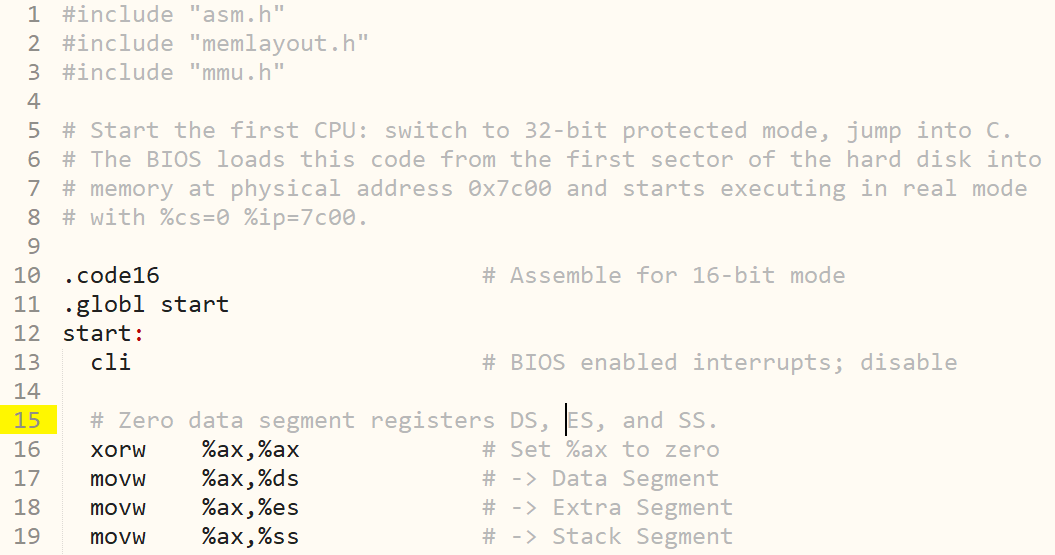
\includegraphics[width=6in]{figures/boot/fig3.png}


但是实模式刚运行完,很多遗留下的一些寄存器的值需要我们整理下,所以我们需要“在16~19行中 将\%ax 置零,然后把这个零值拷贝到三个段寄存器中, 将DS, ES, SS进行清零”。

实模式的东西处理完,我们的重点是要转换到保护模式中去开始真正的工作。为此我们需要打开A20开关, 将32位地址总线打开,使得地址位从20位切换到32位.

关于为什么需要打开A20开关,可以参考文档最后的附录部分.

下面的代码实现了打开A20开关.

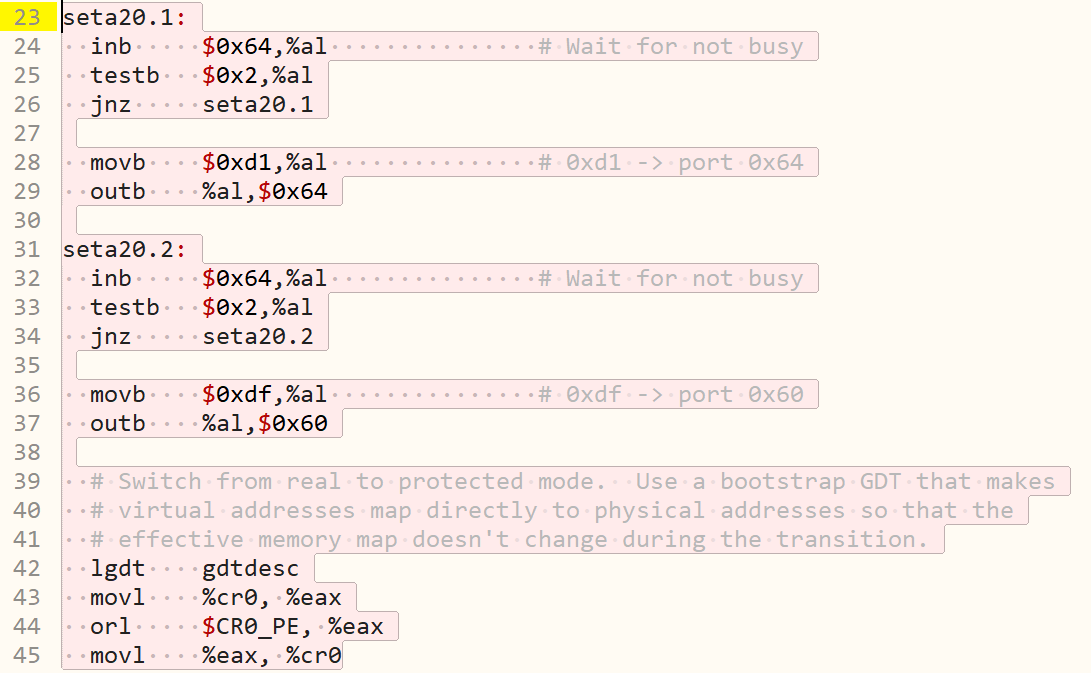
\includegraphics[width=6in]{figures/boot/fig4.png}

接下来加载全局符号表GDT

第42行代码通过引导加载器执行 lgdt指令来把指向 gdt 的指针 gdtdesc加载到全局描述符表(GDT)寄存器中。第44行正式开启保护模式(CR0\_PE=1)接下来第51行处理器还需要将16位模式(因为之前是实模式,所以目前还是处于16位的模式)切换到32位。由于我们没法直接修改 \%cs,所以使用了一个 ljmp 指令ljmp \$(SEG\_KCODE<<3), \$start32。跳转指令会接着在下一行执行,但这样做实际上将 \%cs 指向了 gdt 中的一个代码描述符表项。该描述符描述了一个32位代码段,这样处理器就切换到了32位模式下。

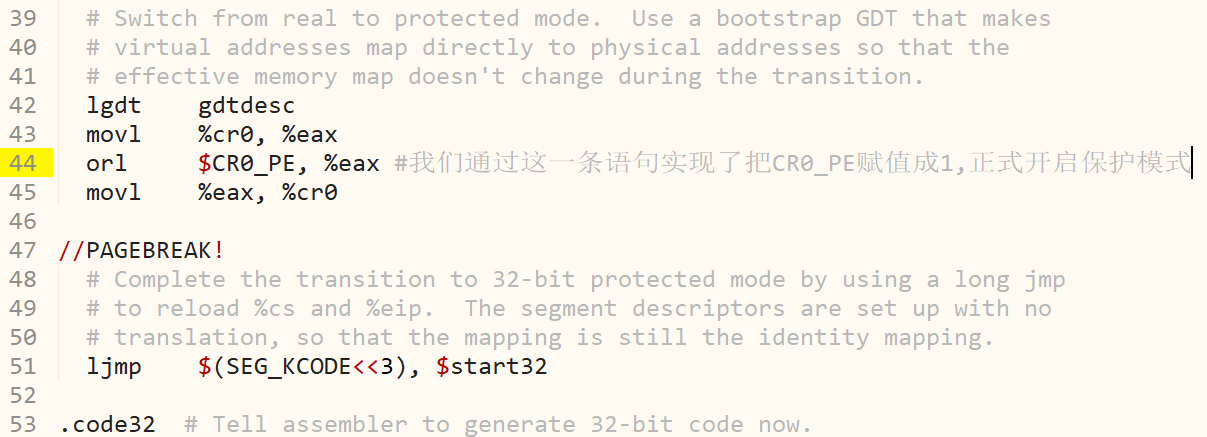
\includegraphics[width=6in]{figures/boot/fig5.png}

接下来完成保护模式之下的初始化数据,然后开始执行bootmain.c代码

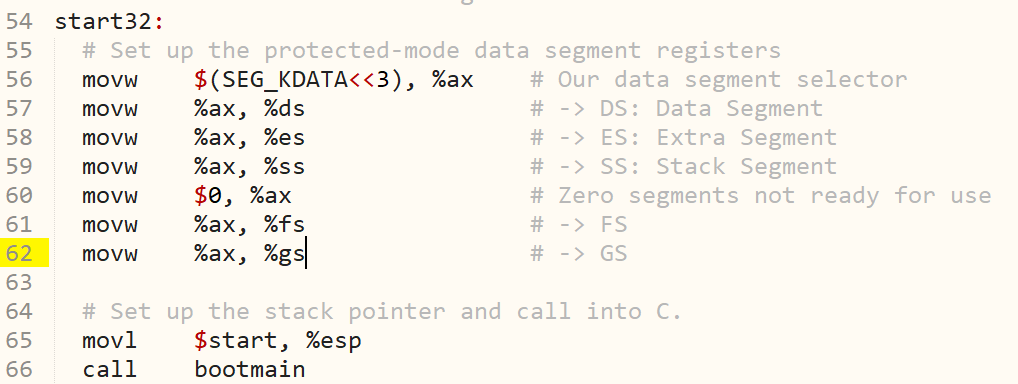
\includegraphics[width=6in]{figures/boot/fig6.png}

\subsubsection{bootmain.c}

在这个文件中主要有四个函数:bootmain、waitdisk、readsect和readseg。其中bootmain是加载内核,其余三个都是对磁盘进行访问的程序。

首先来看一下waitdisk、readsect和readseg。 readseg函数的作用是从磁盘的offset处开始读取count个字符到pa处。在读取数据时是通过调用readsect以扇区为单位进行的。因此在86行保证pa是从一个扇区起始位置开始,因此要对pa进行对齐。readsect是对磁盘进行读取,在读取之前每次调用waitdisk等待磁盘的准备过程,一旦磁盘准备好后就可以进行读取了。

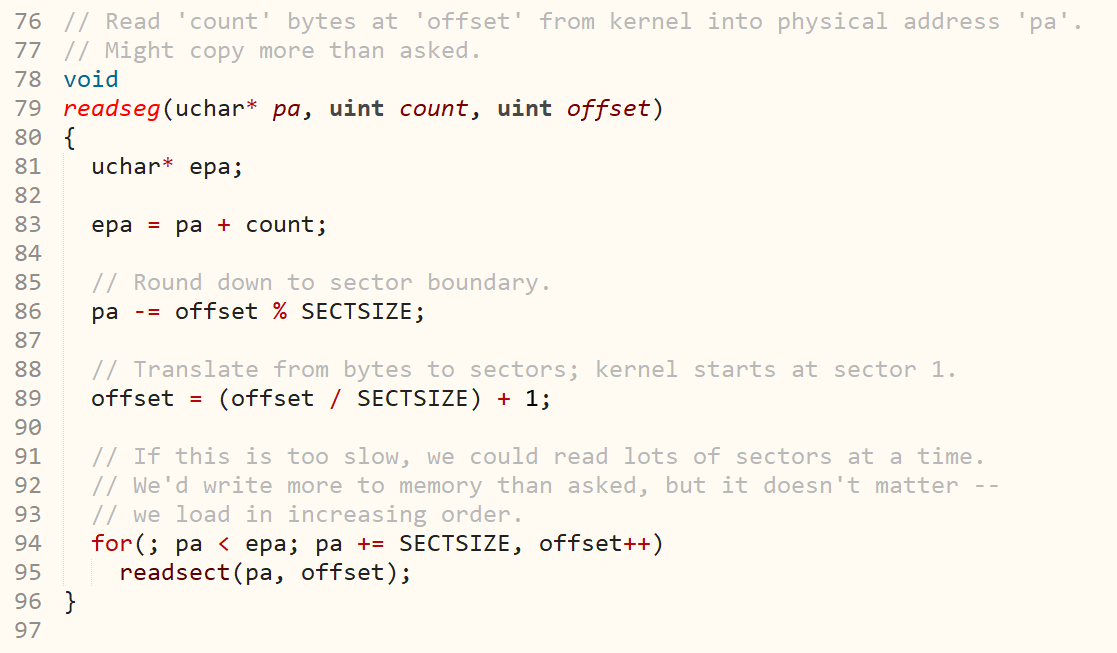
\includegraphics[width=6in]{figures/boot/fig7.png}

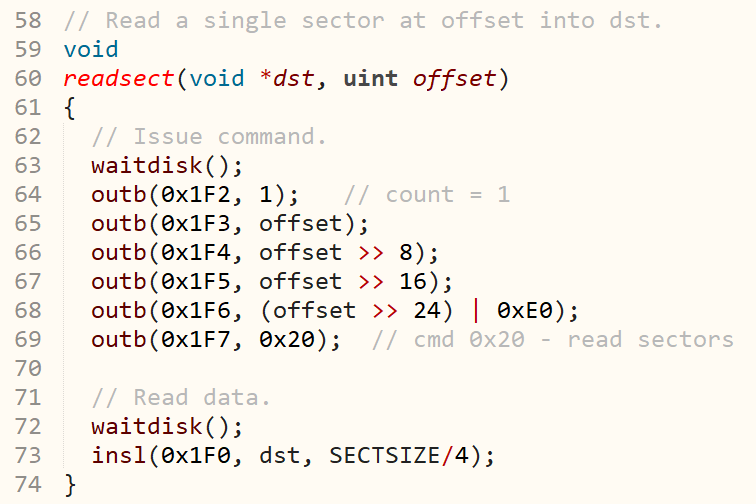
\includegraphics[width=6in]{figures/boot/fig8.png}

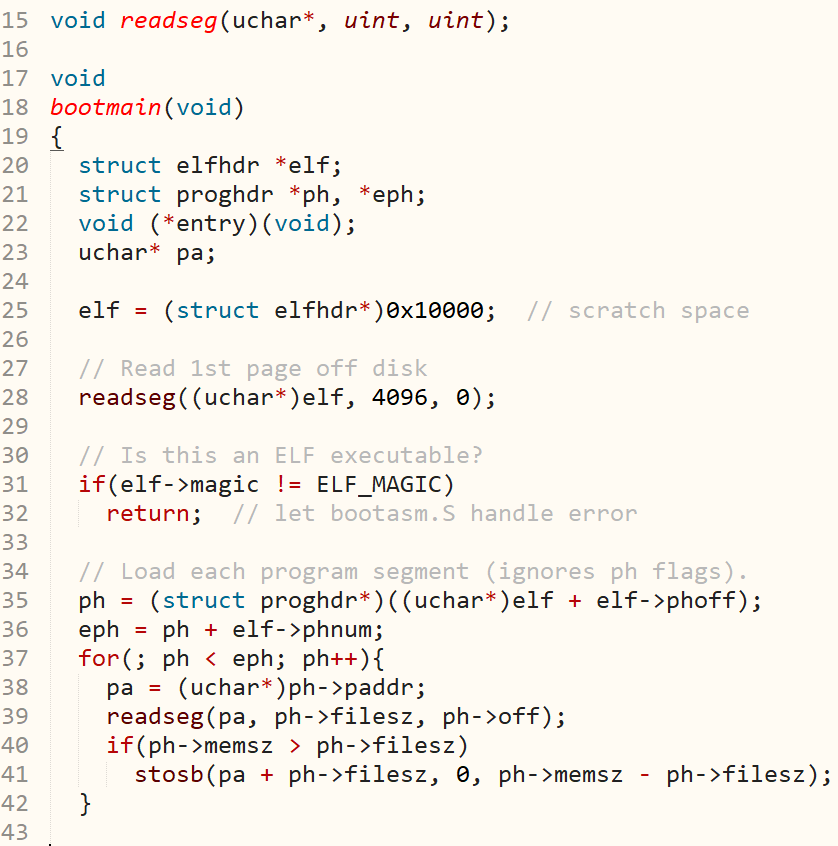
\includegraphics[width=6in]{figures/boot/fig9.png}

然后看一下bootmain过程。bootmain的目的是从磁盘中加载内核到内存中,其中内核是 ELF 格式的二进制文件。为了读取 ELF 头,在第28行bootmain 载入 ELF 文件的前4096字节,并将其拷贝到内存中 0x10000 处。其中包含了ELF执行文件格式的头。从中可以知道读取镜像的大小以及存放的位置

第31行通过 ELF 头检查这是否的确是一个 ELF 文件。

在第39行bootmain 调用 readseg 将数据从磁盘中载入,第41行并调用 stosb 将段的剩余部分置零。stosb使用 x86 指令 rep stosb 来初始化内存块中的每个字节。当完成拷贝后,在第46行bootmain获取内核入口程序的地址,然后进入该入口

bootloader紧接着就是entry开始运行,这个时候x86 的分页硬件在此时还没有开始工作;所以这时的虚拟地址是直接映射到物理地址上的。

boot loader 把 xv6 内核装载到物理地址 0x100000 处。之所以没有装载到内核指令和内核数据应该出现的 0x80100000,是因为小型机器上很可能没有这么大的物理内存。而之所以在 0x100000 而不是 0x0 则是因为地址 0xa0000 到 0x100000 是属于 I/O 设备的。

为了让内核的剩余部分能够运行,entry 的代码设置了页表,将 0x80000000开始的虚拟地址映射到物理地址 0x0 处。

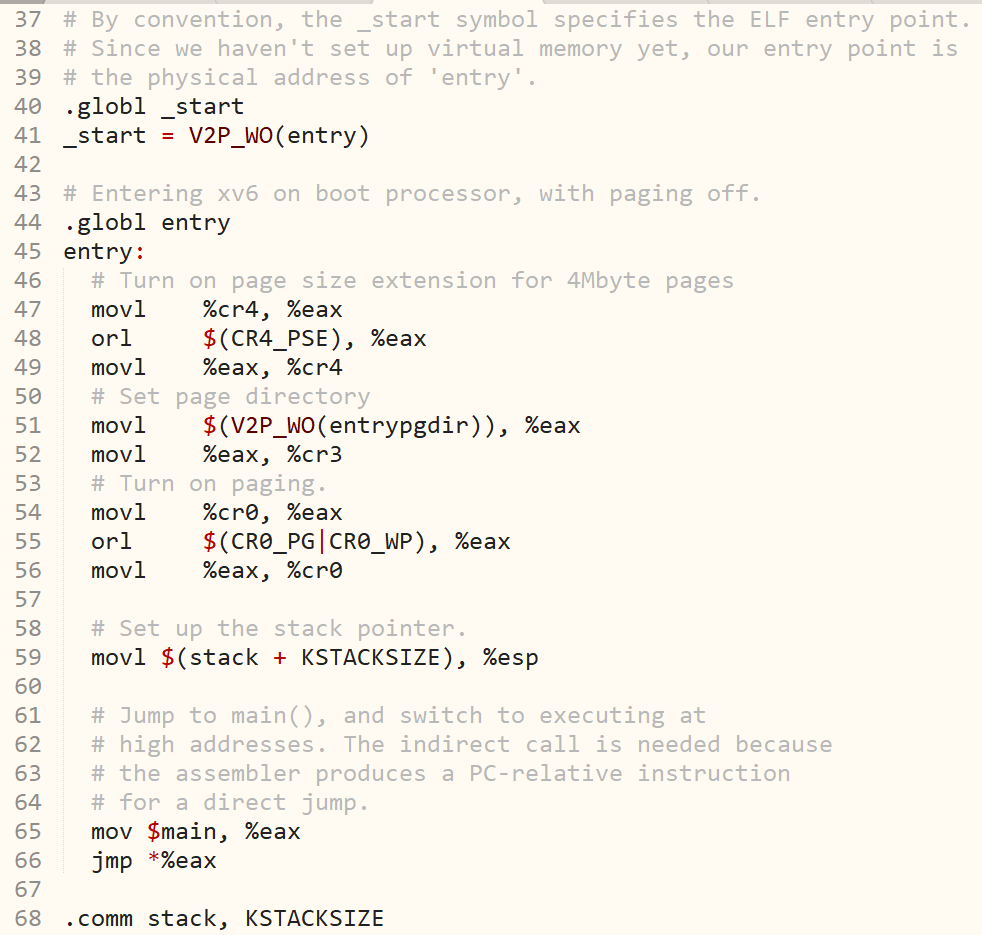
\includegraphics[width=6in]{figures/boot/fig10.png}

Entry 在完成设置页表和栈指针的操作之后,跳转到内核的 C 代码,并在内存的高地址中执行它了。
首先它将栈指针 %esp 指向被用作栈的一段内存。所有的符号包括 stack 都在高地址,所以当低地址的映射被移除时,栈仍然是可用的。
entry 跳转到高地址的 main 代码中。我们必须使用间接跳转,否则汇编器会生成 PC 相关的直接跳转(PC-relative direct jump),而该跳转会运行在内存低地址处的 main。 main 不会返回,因为栈上并没有返回 PC 值。好了,现在内核已经运行在高地址处的函数 main中了。

到现在为止,xv6的引导工作全部完成,接下来开始执行内核代码.
